\section{Research in Context}\label{sr.ric}
\newcommand{\pu}[2]{#1\,+\,#2}
\begin{ric}[b]
  \paragraph{Evidence before this study}
  We adapted and updated a scoping review of HIV transmission modelling studies examining
  the prevention impacts of antiretroviral therapy (ART) cascade scale-up in Sub-Saharan Africa.
  Our search yielded (\pu{prior}{update}) \pu{1367}{373} unique studies, of which:
  \pu{7}{5} examined the prevention impacts of achieving
  the UNAIDS 90-90-90 goals or greater (Table~\ref{tab:ric.refs}).
  Some of these studies considered differences in baseline rates of
  diagnosis, treatment initiation, and/or treatment failure/discontinuation
  --- mainly by sex, age, and occasionally risk.
  Three studies specifically examined scenarios of unequal cascade attainment across subpopulations,
  predicting substantially more infections when subpopulations at higher risk were left behind.
  However, these studies did not maintain consistent overall cascade across scenarios
  --- \ie each scenario reached a different cascade for the population overall ---
  and considered only hypothetical scenarios.
  \paragraph{Added value of this study}
  We developed and calibrated a detailed model of heterosexual HIV transmission
  and observed ART cascade scale-up in Eswatini,
  drawing on population-level and female sex worker (FSW)-specific surveys.
  Eswatini achieved 95-95-95 overall and similar among FSW by 2020.
  We estimated what would have happened if
  overall cascade scale-up had been slower
  (reaching only \casmd by 2020), and
  inequalities in the cascade among FSW and/or clients had not been addressed
  (reaching \caslo by 2020).
  We found that such cascade inequalities
  would have led to 31--128\% additional HIV infections in the overall population by 2020, % MAN
  as compared to equitable scale-up.
  \paragraph{Implications of all the available evidence}
  The population-level prevention benefits of achieving 95-95-95 overall
  are undermined by inequalities in the HIV cascade, especially when
  populations experiencing disproportionate transmission risks are left behind,
  including but not limited to FSW and their clients.
\end{ric}

This section presents results of the scoping review for Box~\ref{ric},
adapted and updated from \cite{Knight2022sr}.
%===================================================================================================
\subsection{Definitions \& Criteria}\label{sr.ric.def}
\begin{table}[h]
  \centering
  \caption{Criteria for inclusion and exclusion}
  \newcommand{\tabitem}{$\bullet$\hspace{.5em}\ignorespaces}
\begin{tabular}{ll}
  \toprule
  Include & Exclude \\
  \midrule
  \multicolumn{2}{l}{\textbf{Publication Type}} \\
  \midrule
  \tabitem English language               & \tabitem non-English \\
  \tabitem peer-reviewed research article & \tabitem non-peer-reviewed \\
                                          & \tabitem review article \\
                                          & \tabitem textbook, grey literature \\
                                          & \tabitem opinions, comments, correspondence \\
                                          & \tabitem conference abstracts and proceedings \\
  \midrule
  \multicolumn{2}{l}{\textbf{Modelling of HIV Transmission}} \\
  \midrule
  \tabitem population-level dynamics               & \tabitem only within-host/cellular/protein modelling \\
  \tabitem sexual HIV transmission model           & \tabitem no sexual HIV transmission modelled \\
  \tabitem non-linear HIV transmission model\tn{*} & \tabitem HIV transmission model is linear \\
                                                   & \tabitem HIV incidence is fixed or imported \\
  \midrule
  \multicolumn{2}{l}{\textbf{Context \& Objectives}} \\
  \midrule
  \tabitem any region in Sub-Saharan Africa (SSA)\tn{*} & \tabitem only regions outside SSA\tn{*}\\
                                                        & \tabitem only theoretical context \\
  \tabitem includes 90-90-90+ scenario\tn{*}            & \tabitem no 90-90-90+ scenario\tn{*}   \\
  \tabitem includes base-case reflecting status quo     & \tabitem no base-case scenario \\
  \tabitem report prevention impacts of 90-90-90+\tn{*} & \tabitem did not report ART prevention impacts\tn{*} \\
                                                        & \tabitem intervention/budget optimization \\
                                                        & \tabitem viral load monitoring or regimen switching \\
  \bottomrule
\end{tabular}
\floatfoot{\tnt[*]{See definitions in \ref{sr.ric.def}.}}

  \label{tab:ric.crit}
\end{table}
Table~\ref{tab:ric.crit} gives the inclusion/exclusion criteria for our review,
while key definitions are given below:
\paragraph{Non-linear model}
Any model where:
the number of infections projected at time $t$ is an iterative function of
the number of infections previously projected by the model before time $t$.
\paragraph{Sub-Saharan Africa} (SSA)
any country in the UN regions of East, South, Central, and West Africa, plus South Sudan
(see Table~\ref{tab:ric.search} for full country list).
\paragraph{90-90-90+ scenario}
Among all people living with HIV (regardless of CD4 count):
90+\% are diagnosed, of whom 90+\% are on ART, of whom 90+\% are virally suppressed
--- or 73+\% are effectively modelled as virally suppressed ---
achieved for the population overall by any year,
and without any other interventions beyond status quo.
We further distinguish between
\emph{named} 90-90-90+ scenarios and
\emph{effectively} 90-90-90+ scenarios based on modelled rates.
\paragraph{Quantified prevention impacts}
HIV incidence rate reduction or cumulative infections averted among the whole population
in 90-90-90+ \vs status quo scenario over any time horizon.
%===================================================================================================
\subsection{Search Strategy \& Hits}\label{sr.ric.search}
We searched MEDLINE and EMBASE via Ovid on:
2020 March 20 (studies published before 2020) and
2023 November 23 (studies published in/after 2020).
Table~\ref{tab:ric.search} gives the search terms and hits from each search, where
\texttt{term/} denotes a MeSH term, and
\texttt{.mp} searches the main text fields, including title, abstract, and heading words.
Duplicate studies were removed automatically by Ovid.
Figure~\ref{fig:api.prisma} illustrates the PRISMA diagram for study identification.
\begingroup\footnotesize\singlespace
\begin{longtable}{lrp{.8\textwidth}}
  \caption{Search terms and hits}
  \label{tab:ric.search} \\
  \toprule & Hits & Term \\ \midrule \endfirsthead
  \midrule \endhead \midrule \endfoot \bottomrule \endlastfoot
   \st{M1} &  \num{259932} & \st{model, theoretical/} \\
   \st{M2} &  \num{357388} & \st{model, biological/} \\
   \st{M3} &  \num{354078} & \st{computer simulation/} \\
   \st{M4} &  \num{210102} & \st{patient-specific modeling/} \\
   \st{M5} &   \num{84649} & \st{monte carlo method/} \\
   \st{M6} &   \num{70865} & \st{exp stochastic processes/} \\
   \st{M7} &  \num{621337} & \st{(model* ADJ3 (math* OR transmission OR dynamic* OR epidemi* OR compartmental OR deterministic OR individual OR agent OR network OR infectious disease* OR markov OR dynamic* OR simulat*)).mp.} \\
   \st{M8} & \num{1648338} & \st{OR/ M1-M7} \\
  \midrule
   \st{H1} &  \num{331119} & \st{exp HIV/} \\
   \st{H2} &  \num{748853} & \st{exp HIV infections/} \\
   \st{H3} &  \num{880774} & \st{(HIV OR HIV1* OR HIV2* OR HIV-1* OR HIV-2*).mp.} \\
   \st{H4} &  \num{426755} & \st{hiv infect*.mp.} \\
   \st{H5} &  \num{627422} & \st{(human immun*deficiency virus OR human immun* deficiency virus).mp.} \\
   \st{H6} &  \num{234482} & \st{exp Acquired Immunodeficiency Syndrome/} \\
   \st{H7} &  \num{249998} & \st{(acquired immun*deficiency syndrome OR acquired immun* deficiency syndrome).mp.} \\
   \st{H8} & \num{1105191} & \st{OR/ H1-H7} \\
  \midrule
   \st{G1} &    \num{4550} & \st{Angola/ OR Angola.mp.} \\
   \st{G2} &   \num{11475} & \st{Benin/ OR Benin.mp.} \\
   \st{G3} &    \num{7688} & \st{Botswana/ OR Botswana.mp.} \\
   \st{G4} &   \num{13091} & \st{Burkina Faso/ OR Burkina Faso.mp.} \\
   \st{G5} &    \num{2713} & \st{Burundi/ OR Burundi.mp.} \\
   \st{G6} &   \num{21726} & \st{Cameroon/ OR Cameroon.mp.} \\
   \st{G7} &    \num{1598} & \st{Cape Verde/ OR Cape Verde.mp.} \\
   \st{G8} &   \num{28956} & \st{Central African Republic/ OR Central African Republic.mp. OR CAR.ti.} \\
   \st{G9} &    \num{4129} & \st{Chad/ OR Chad.mp.} \\
  \st{G10} &    \num{1320} & \st{Comoros/ OR Comoros.mp.} \\
  \st{G11} &   \num{18397} & \st{Democratic Republic of the Congo/ OR Democratic Republic of the Congo.mp. OR DRC.mp.} \\
  \st{G12} &    \num{1209} & \st{Djibouti/ OR Djibouti.mp.} \\
  \st{G13} &    \num{1410} & \st{Equatorial Guinea/ OR Equatorial Guinea.mp.} \\
  \st{G14} &    \num{1941} & \st{Eritrea/ OR Eritrea.mp.} \\
  \st{G15} &   \num{64626} & \st{Ethiopia/ OR Ethiopia.mp.} \\
  \st{G16} &    \num{5383} & \st{Gabon/ OR Gabon.mp.} \\
  \st{G17} &    \num{7939} & \st{Gambia/ OR Gambia.mp.} \\
  \st{G18} &   \num{37148} & \st{Ghana/ OR Ghana.mp.} \\
  \st{G19} &  \num{370653} & \st{Guinea/ OR Guinea.mp.} \\
  \st{G20} &    \num{3084} & \st{Guinea-Bissau/ OR Guinea-Bissau.mp.} \\
  \st{G21} &   \num{11852} & \st{Cote d'Ivoire/ OR Cote d'Ivoire.mp. OR Ivory Coast.mp.} \\
  \st{G22} &   \num{60705} & \st{Kenya/ OR Kenya.mp.} \\
  \st{G23} &    \num{2372} & \st{Lesotho/ OR Lesotho.mp.} \\
  \st{G24} &    \num{5259} & \st{Liberia/ OR Liberia.mp.} \\
  \st{G25} &   \num{13940} & \st{Madagascar/ OR Madagascar.mp.} \\
  \st{G26} &   \num{22145} & \st{Malawi/ OR Malawi.mp.} \\
  \st{G27} &   \num{11543} & \st{Mali/ OR Mali.mp.} \\
  \st{G28} &    \num{1997} & \st{Mauritania/ OR Mauritania.mp.} \\
  \st{G29} &    \num{2928} & \st{Mauritius/ OR Mauritius.mp.} \\
  \st{G30} &   \num{11416} & \st{Mozambique/ OR Mozambique.mp.} \\
  \st{G31} &    \num{5216} & \st{Namibia/ OR Namibia.mp.} \\
  \st{G32} &   \num{43198} & \st{Niger/ OR Niger.mp.} \\
  \st{G33} &  \num{105242} & \st{Nigeria/ OR Nigeria.mp.} \\
  \st{G34} &   \num{17810} & \st{Republic of the Congo/ OR Republic of the Congo.mp. OR Congo-Brazzaville.mp.} \\
  \st{G35} &    \num{1860} & \st{Reunion/} \\
  \st{G36} &   \num{10849} & \st{Rwanda/ OR Rwanda.mp.} \\
  \st{G37} &     \num{488} & \st{"Sao Tome and Principe"/ OR "Sao Tome and Principe".mp.} \\
  \st{G38} &   \num{19552} & \st{Senegal/ OR Senegal.mp.} \\
  \st{G39} &    \num{2027} & \st{Seychelles/ OR Seychelles.mp.} \\
  \st{G40} &    \num{7333} & \st{Sierra Leone/ OR Sierra Leone.mp.} \\
  \st{G41} &    \num{6180} & \st{Somalia/ OR Somalia.mp.} \\
  \st{G42} &  \num{145351} & \st{South Africa/ OR South Africa.mp.} \\
  \st{G43} &    \num{1909} & \st{South Sudan/ OR South Sudan.mp.} \\
  \st{G44} &   \num{26487} & \st{Sudan/ OR Sudan.mp.} \\
  \st{G45} &    \num{3261} & \st{Swaziland/ OR Swaziland.mp. OR Eswatini/ OR Eswatini.mp.} \\
  \st{G46} &   \num{43118} & \st{Tanzania/ OR Tanzania.mp.} \\
  \st{G47} &    \num{4746} & \st{Togo/ OR Togo.mp.} \\
  \st{G48} &   \num{50642} & \st{Uganda/ OR Uganda.mp.} \\
  \st{G49} &   \num{17842} & \st{Zambia/ OR Zambia.mp.} \\
  \st{G50} &   \num{19262} & \st{Zimbabwe/ OR Zimbabwe.mp.} \\
  \st{G51} &  \num{625159} & \st{exp africa south of the sahara/ OR sub-saharan.mp. OR south of the sahara.mp.} \\
  \st{G52} & \num{1191770} & \st{OR/ G1-G51} \\
  \midrule
   \st{X1} & \num{2777} & \st{M8 AND H8 AND G52} \\
   \st{X2} & \num{2740} & \st{X1 NOT animal/} \\
   \st{X3} & \num{2733} & \st{limit X2 to english language} \\
   \st{X5} & \num{1740} & \st{remove duplicates from X4}    \\
\end{longtable}
\endgroup

\begin{figure}[h]
  \centering
  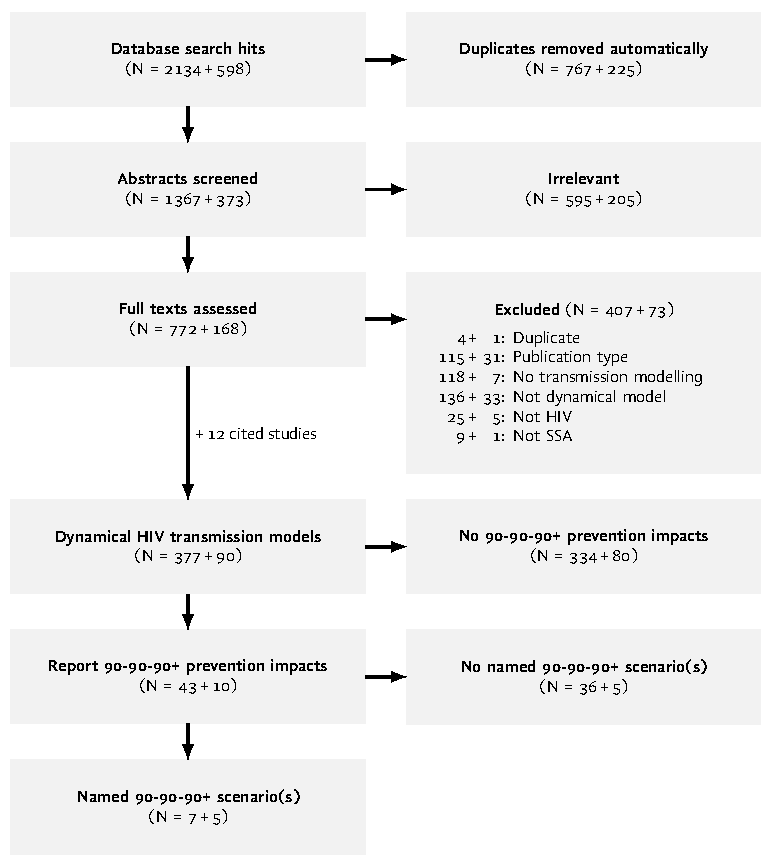
\includegraphics[scale=1]{api.prisma}
  \caption{PRISMA diagram for identifying studies modelling the prevention impacts of 90-90-90+}
  \label{fig:api.prisma}
\end{figure}
%===================================================================================================
\subsection{Included Studies}\label{sr.ric.refs}
Table~\ref{tab:ric.refs} summarizes the
characteristics of included studies with named 90-90-90+ scenarios.
\begin{landscape}
\begin{table}
  \caption{Characteristics of studies modelling prevention impacts in named 90-90-90+ scenarios}
  \centering
  \begin{tabular}{rllllllll}
  \toprule
  &&& \multicolumn{3}{c}{Status Quo Rate Diffs\tn{12}} & \multicolumn{2}{c}{90-90-90+ Scenarios} & \\
  \cmidrule(rl){4-6}\cmidrule(rl){7-8}
  Ref                         & Model Name & Strata\tn{1} & Diag & Init & Supp & Prioritized & Left Behind & Modelled Context \\
  \midrule
  \citet{Hontelez2016}        & STDSIM     & SARK &  S  &  S  & --- & ---  & --- & Sub-Saharan Africa \\
  \citet{Maheu-Giroux2017art} & ---        & SARK & SAK & --- &  K  &  K   &  K  & C\^{o}te d'Ivoire \\
  \citet{Volz2017}            & ---        &  SK  &  K  &  K  & --- &  K   & --- & Nigeria \\
  \citet{Bansi-Matharu2018}   & Synthesis  & SARK & SAR &  S  & --- & ---  & --- & Zimbabwe \\
  \citet{Stuart2018ft}        & Optima     & SARK & SAK & SAK & --- & ---  & --- & Johannesburg, South Africa \\
  \citet{Abuelezam2019}       & CDM        & SARK & --- & --- & --- & SARK & --- & South Africa \\
  \citet{Reidy2019}           & Goals      & SRK  &  S  &  S  & --- & ---  &  S  & Kenya; South Africa; Uganda; Zimbabwe \\
  \citet{Akullian2020}        & EMOD       & SARK & SA  & SA  & --- &  A   & --- & Eswatini \\
  \citet{Marukutira2020}      & Optima     &  SM  & SM  & SM  &  M  & ---  &  M  & Botswana \\
  \citet{Kripke2022}          & Goals      & SRK  &  S  &  S  & --- & ---  & --- & Lesotho; Mozambique; Uganda \\
  \citet{LuongNguyen2022}     & ---     & R\tn{3} & --- & --- & --- & ---  & --- & Kenya \\
  \citet{Probert2022}         & PopART-IBM & SAR  &  S  & --- &  S  & ---  & --- & Zambia; South Africa \\
  \bottomrule
\end{tabular}
\floatfoot{
  \tnt[1]{S: sex; A: age; R: risk; K: any key population(s); M: migrants};
  \tnt[2]{Differences in rates of diagnosis, ART initiation, or viral suppression
  (including treatment failure, discontinuation, loss-to-follow-up)};
  \tnt[3]{Risk groups were defined by age/sex}.}

  \label{tab:ric.refs}
\end{table}
\end{landscape}
